\begin{figure}[h]
	\centering
	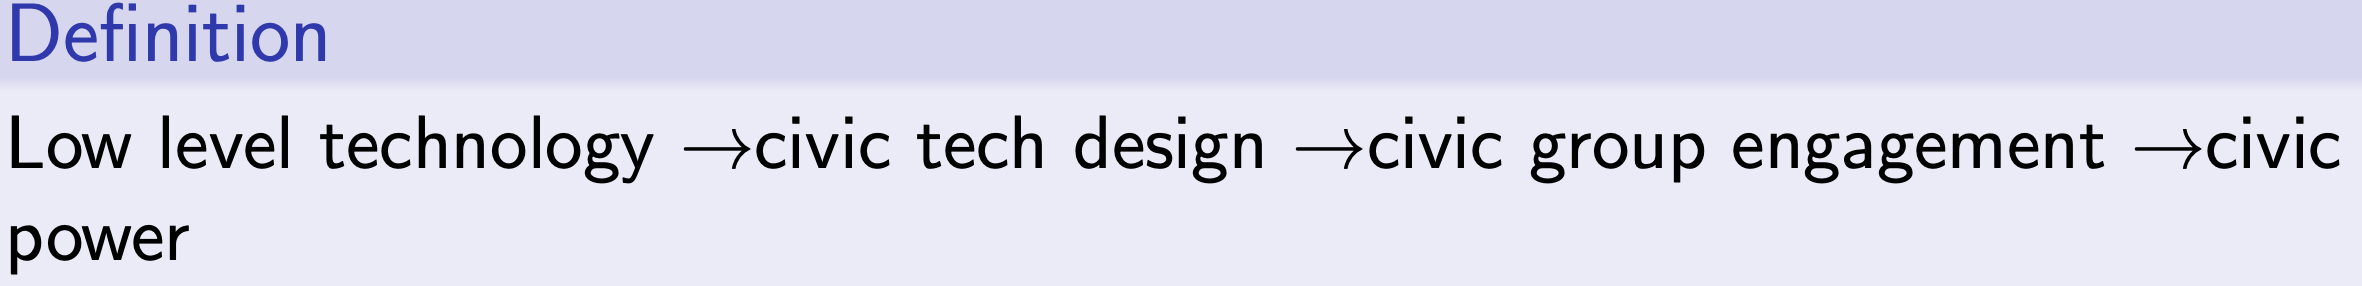
\includegraphics[scale=0.3]{images/taxonomy-pipeline}
	\caption{Pipeline taxonomy}
	\label{fig:taxonomy-pipeline}
\end{figure}

The diagram within Figure {fig:taxonomy-pipeline} represnts an alternative, 'pipeline', taxonomy of civic technology projects.
On the far left hand side of the diagram, can be found low Level technologies, such as servers or the accessibility of open web networks - important when considering civic technologies in countries with restrictive web practicies.
Moving forward to the right, the taxonomy addresses the design of individual civic tech projects, including the type of content that the offer.	
The taxonomy then encompasses the types of engagement such projects offer, particulary with regard to group membership.
Lastly, it finishes with a phrase coined by Tom Steinberg (the founded of My Society), namely, civic power. 
That is, what types of civic power does a project engender.
  